% This LaTeX document needs to be compiled with XeLaTeX.
\documentclass[10pt]{article}
\usepackage{ucharclasses}
\usepackage{graphicx}
\usepackage[export]{adjustbox}
\graphicspath{ {./images/} }
\usepackage{hyperref}
\hypersetup{colorlinks=true, linkcolor=blue, filecolor=magenta, urlcolor=cyan,}
\urlstyle{same}
\usepackage[fallback]{xeCJK}
\usepackage{polyglossia}
\usepackage{fontspec}
\setCJKmainfont{Noto Serif CJK TC}

\setmainlanguage{german}
\setotherlanguages{czech}
\newfontfamily\lgcfont{CMU Serif}
\setDefaultTransitions{\lgcfont}{}

\title{Bachelor of Science (BSc) in Informatik Modul Software-Entwicklung 1 (SWEN1) }

\author{}
\date{}


\begin{document}
\maketitle
\section*{V3 - Persistenz}
SWEN1/PM3 Team:\\
R. Ferri (feit), D. Liebhart (lieh), K. Bleisch (bles), G. Wyder (wydg)

\section*{Um was geht es?}
\begin{itemize}
  \item Wie kann ich meine Java Objekte dauerhaft speichern?
\end{itemize}

Java

\begin{itemize}
  \item Welche Arten von Datenspeicherung gibt es?
  \item Welche Design Patterns stehen für die Realisierung von Persistenz in einer Applikation zur Verfügung?
  \item Wie kann ich mit Hilfe von den Java APIs JDBC (Java Database Connectivity) und JPA (Java Persistence API) meine Objekte dauerhaft in einer Datenbank speichern?
\end{itemize}

\section*{Applikation}
\begin{verbatim}
DB API
\end{verbatim}

\begin{center}
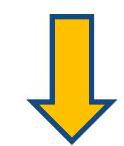
\includegraphics[width=\linewidth]{images/2025_01_02_5ba1dc702e9f94ba8e06g-02}
\end{center}

Treiber

\section*{Lernziele LE 12 - Persistenz}
\begin{itemize}
  \item Sie sind in der Lage
  \item die Varianten der Datenspeicherung zu nennen,
  \item die unterschiedlichen Design Patterns für die Persistenz zu erklären,
  \item mit Hilfe des Design Patterns DAO (Data Access Object) und JDBC eine Persistenz in Java umzusetzen,
  \item mit JPA ein Objekt-Relationales-Mapping (O/R-Mapping) in Java anzuwenden.
\end{itemize}

\section*{1. Einführung in Persistenz}
\begin{enumerate}
  \setcounter{enumi}{1}
  \item Design-Optionen für Persistenz
  \item Persistenz mit JDBC
  \item O/R-Mapping mit DAO
  \item O/R-Mapping mit JPA
  \item Wrap-up und Ausblick
\end{enumerate}

\section*{Problemstellung Persistenz (1/2)}
\begin{itemize}
  \item In vielen Applikationen müssen unterschiedliche Daten verarbeitet, verwaltet und dauerhaft, d.h. über das Programmende hinaus gesichert werden.
  \item Letzteres bezeichnet man als Persistenz.
  \item Die dauerhafte Speicherung erfolgt in Datenbankmanagementsystemen (DBMS).
  \item Übliche Datenbanksysteme sind sogenannte Relationale Datenbanksysteme (RDBMS) und sogenannte NoSQL-Datenbanken.
  \item NoSQL-Datenbanken speichern Daten ohne fixes Schema und in verschiedenen Formaten (Dokument Stores, Key-Value Stores, Graph DB, ...).
\end{itemize}

\section*{Problemstellung Persistenz (2/2)}
\begin{itemize}
  \item Die Abbildung zwischen Objekten und Datensätzen in Tabellen einer relationalen Datenbank wird auch als O/R-Mapping (Object Relational Mapping, ORM) bezeichnet.
  \item Verhältnismässig viel Java-Code wird benötigt, um die Datensätze des Ergebnisses zu verarbeiten und in Java-Objekte zu transformieren.
  \item Es besteht ein Strukturbruch (engl. Impedance Mismatch) aufgrund der unterschiedlichen Repräsentationsformen von Daten (flache Tabellenstruktur -Java-Objekte).
\end{itemize}

Objektorientiertes Programm\\
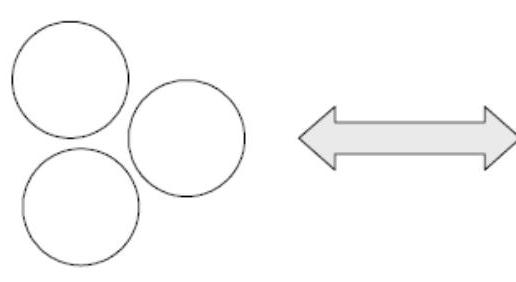
\includegraphics[width=\linewidth]{images/2025_01_02_5ba1dc702e9f94ba8e06g-06}

Relationale Datenbank\\
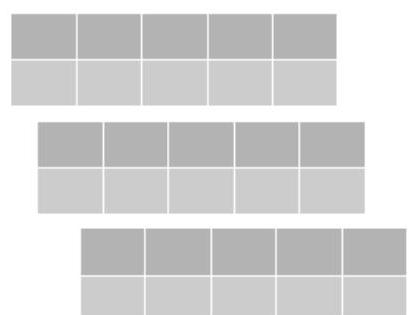
\includegraphics[width=\linewidth]{images/2025_01_02_5ba1dc702e9f94ba8e06g-06(1)}

\section*{Denkpause}
\section*{Aufgabe 12.1 (5')}
Diskutieren Sie in Murmelgruppen folgende Frage:

\begin{itemize}
  \item Was ist aktuell die vorherrschende Technologie zum Speichern von Daten im Enterprise-Umfeld?
  \item Recherchieren Sie dazu unter \href{https://db-engines.com/en/ranking}{https://db-engines.com/en/ranking}.
  \item Was sind die Gründe für dieses Ranking?
\end{itemize}

\begin{enumerate}
  \item Einführung in Persistenz
  \item Design-Optionen für Persistenz
  \item Persistenz mit JDBC
  \item O/R-Mapper mit DAO
  \item O/R-Mapper mit JPA
  \item Wrap-up und Ausblick
\end{enumerate}

\section*{Herausforderung: Der O/R-Mismatch (1/2)}
\begin{itemize}
  \item Der O/R-Mismatch ist ein Fakt.
  \item Der O/R-Mismatch folgt aus konzeptionellen Unterschieden der zugrundeliegenden Technologien.
  \item Es gibt viele verschiedene Möglichkeiten (Patterns) den O/R-Mismatch zu überwinden.
  \item Active Record, O/R-Mapping resp. O/R-Mapping Frameworks oder Repositories (aus Domain Driven Design, DDD) sind ein möglicher Lösungsansatz.
\end{itemize}

\section*{Herausforderung: Der O/R-Mismatch (2/2)}
\begin{itemize}
  \item Typen-Systeme
  \item Null
  \item Datum/Zeit
  \item Abbildung von Beziehungen
  \item Richtung
  \item Mehrfachbeziehungen
  \item Vererbung
  \item Identität
  \item Objekte haben eine implizite Identität
  \item Relationen haben eine explizite Identität (Primary Key)
  \item Transaktionen
\end{itemize}

\section*{JDBC: Java Database Connectivity (1997)}
School of Engineering

\begin{itemize}
  \item JDBC verbindet die Objektwelt mit der relationalen Datenbankwelt
  \item Herausforderung: Objekte vs. Tabellen,
  \item Verschiedene Datentypen etc.
  \item Die Programmierung ist aufwändig\\
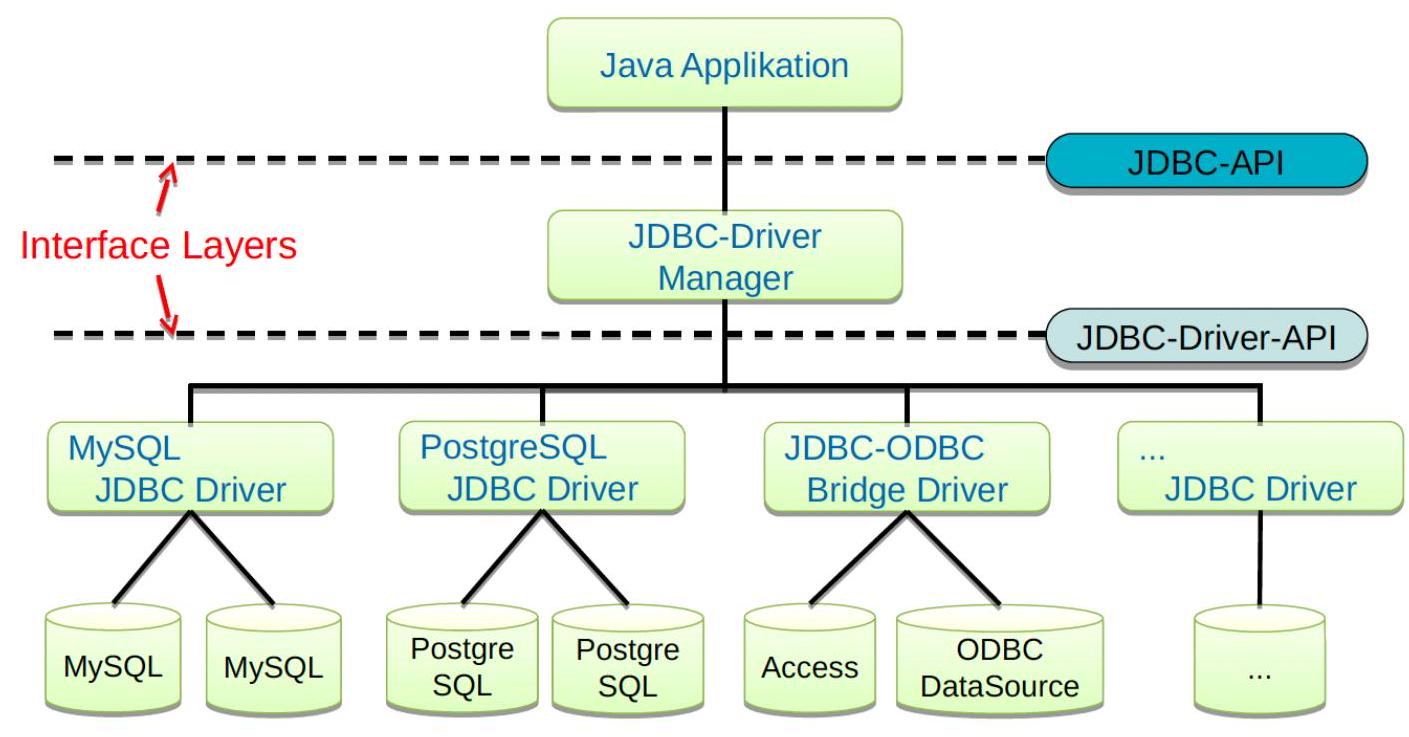
\includegraphics[width=\linewidth]{images/2025_01_02_5ba1dc702e9f94ba8e06g-11}\\
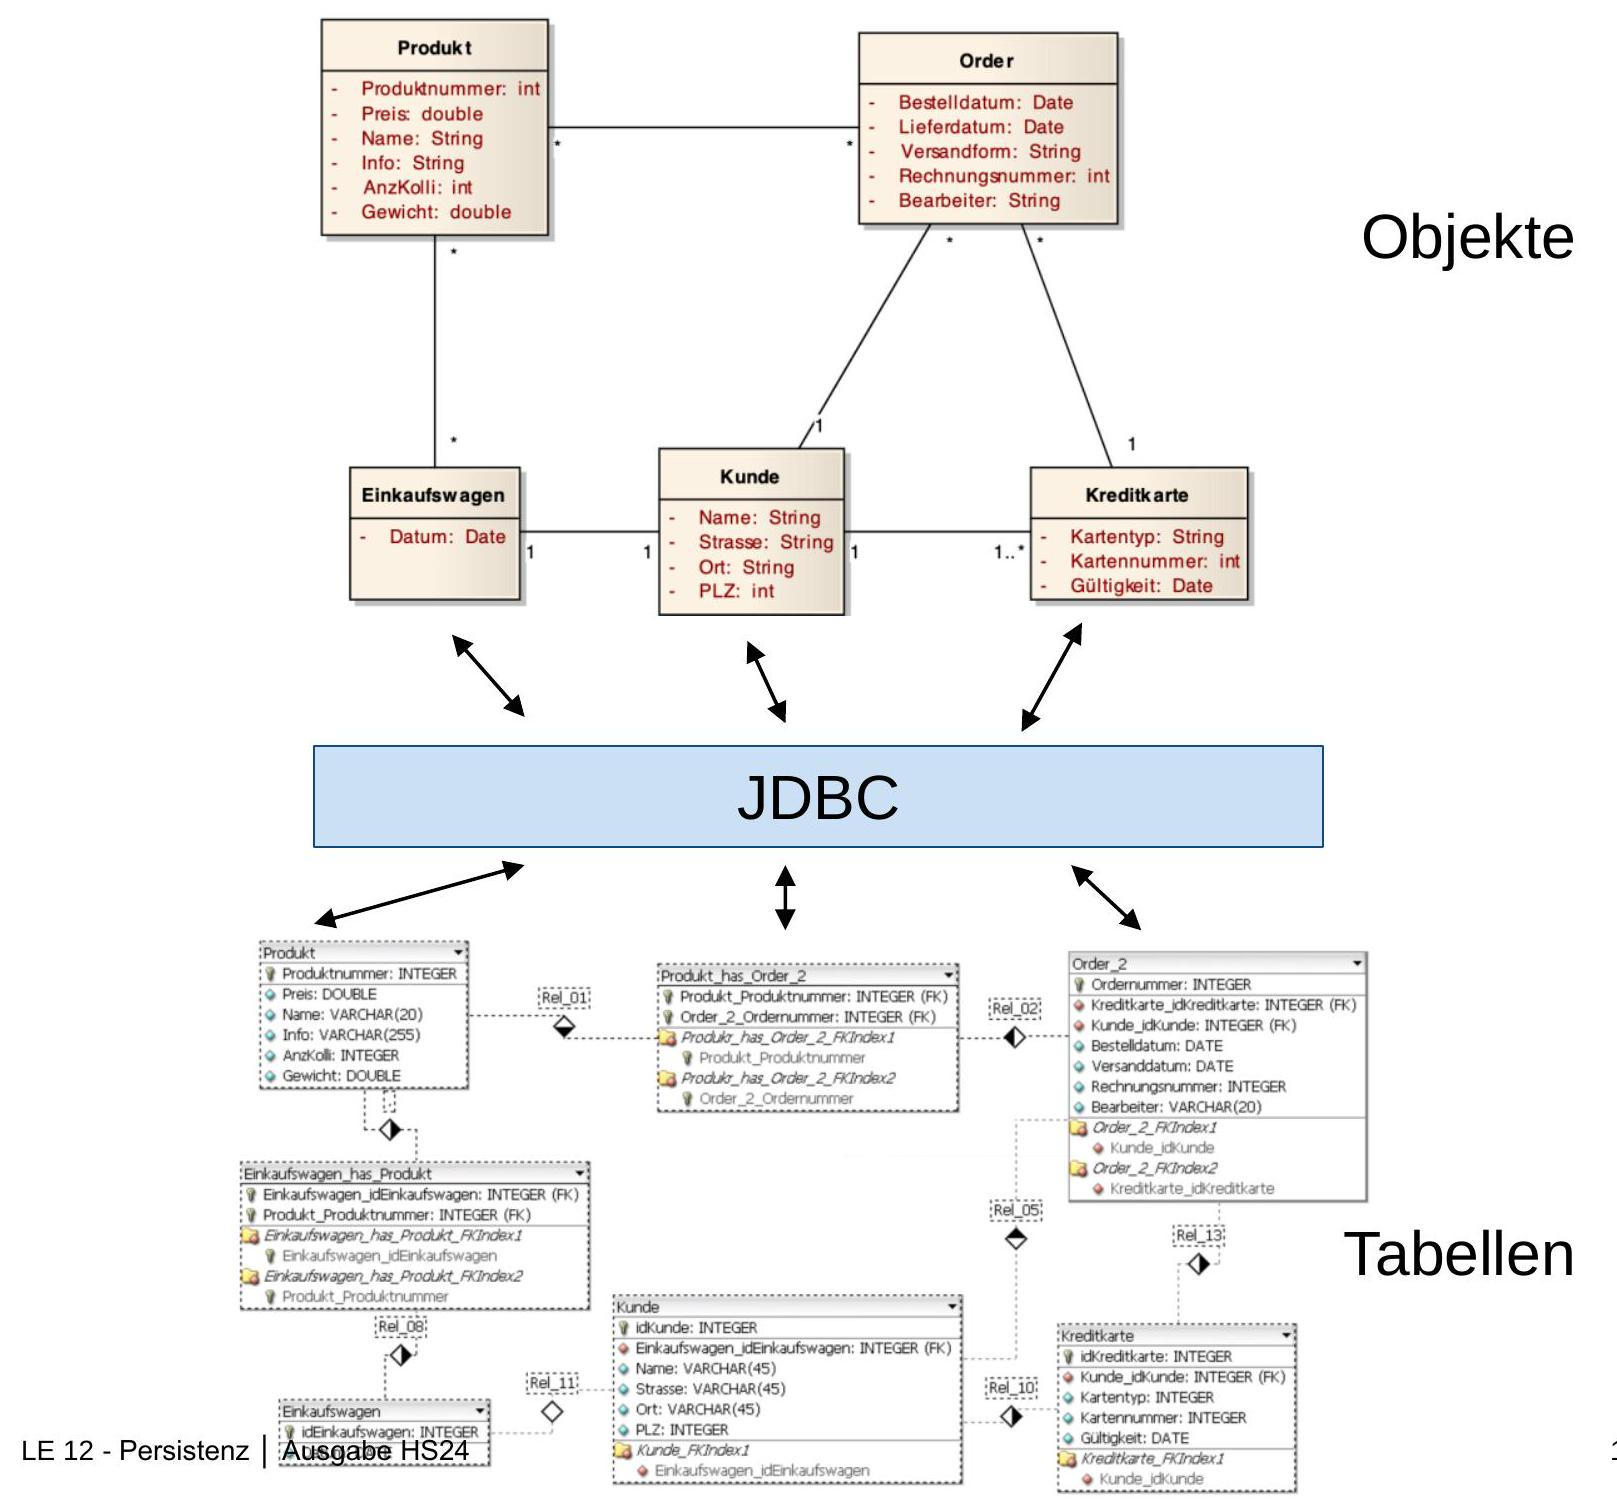
\includegraphics[width=\linewidth]{images/2025_01_02_5ba1dc702e9f94ba8e06g-11(1)}
\end{itemize}

\section*{Design Pattern für Persistenz}
Für eine Persistenz-Strategie muss eine Entscheidung getroffen werden, wo die Zuordnung (Mapping) zwischen Objekten und Tabellen stattfinden soll:

\begin{itemize}
  \item Active Record (Anti Pattern): Jede Entität ist selber dafür zuständig
  \item Data Access Object (DAO): Abstrahiert und kapselt den Zugriff auf die Datenquelle
  \item O/R Data Mapper: Separate Klasse für das Mapping oder Einsatz eines ORM
  \item Zugriffscode auf Datenbank ist in der Domänenklasse
  \item Wrapper für eine Zeile einer Datenbanktabelle
  \item Spiegelt die Datenbankstruktur
  \item Enthält Daten und Verhalten
  \item Fachlichkeit und Technik alles in einer Klasse (GRASP: Information Expert?)
  \item Schlechte Testbarkeit der Domänenlogik ohne Datenbank\\
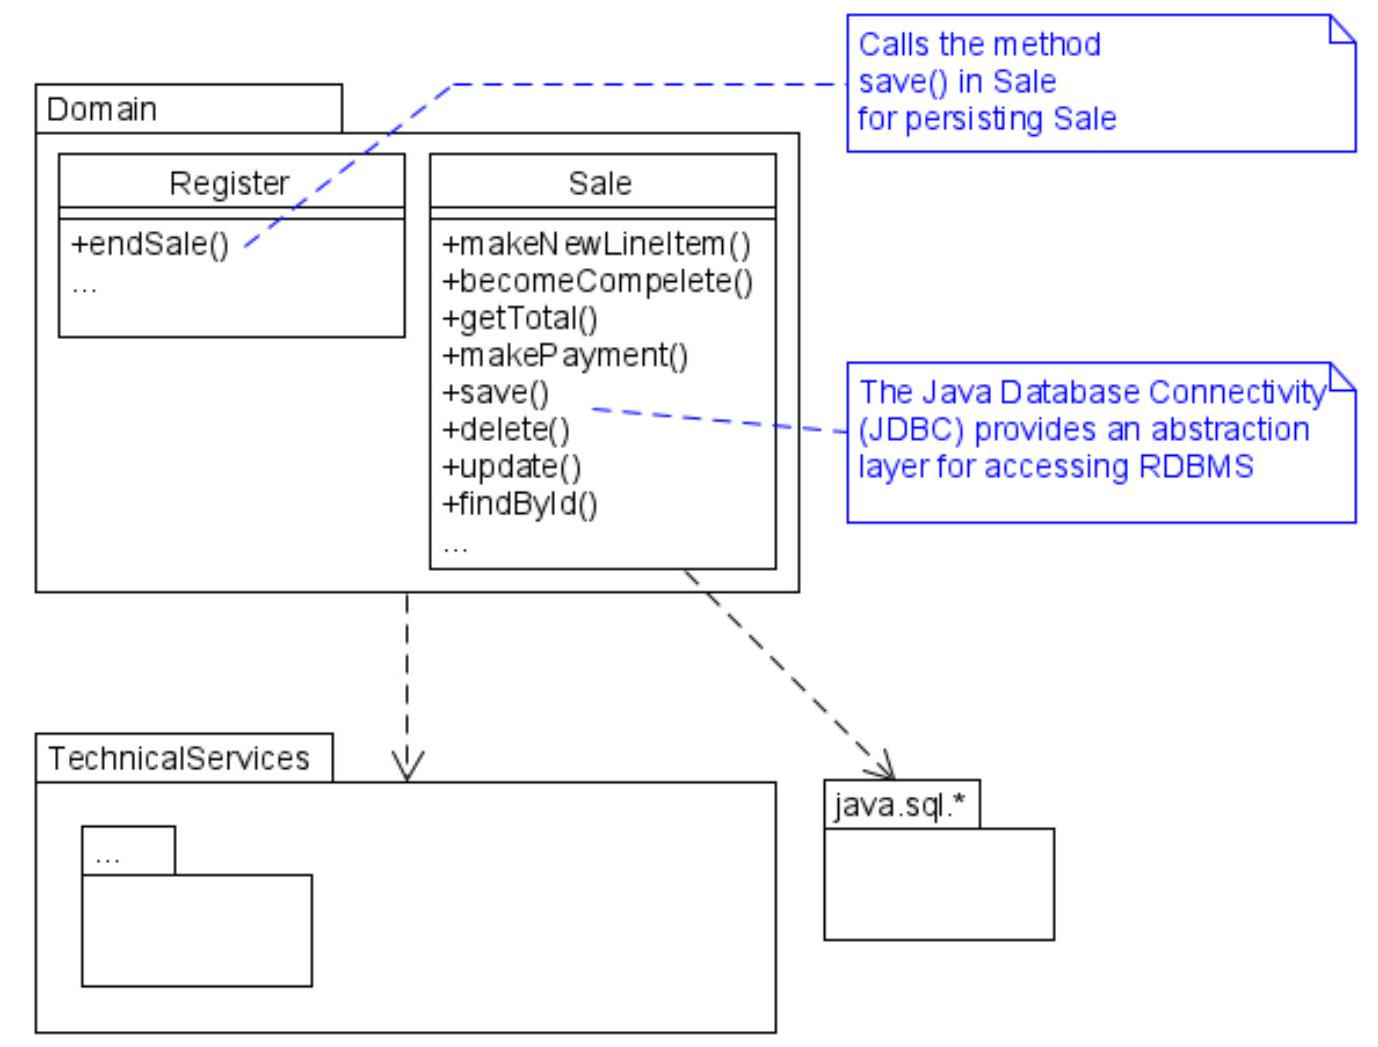
\includegraphics[width=\linewidth]{images/2025_01_02_5ba1dc702e9f94ba8e06g-13}
  \item Schlechte Wartbarkeit und Erweiterbarkeit (No separation of concerns!)
\end{itemize}

\section*{O/R-Mapping von Hand mit Hilfe eines Data Access Objects (DAO)}
\begin{itemize}
  \item Trennung von Fachlichkeit und Technik (Domänenklasse hat hohe Kohäsion)
  \item Gute Testbarkeit und Mocking der Persistenz
  \item Bevorzugtes Design ohne Einsatz eines O/RMappers\\
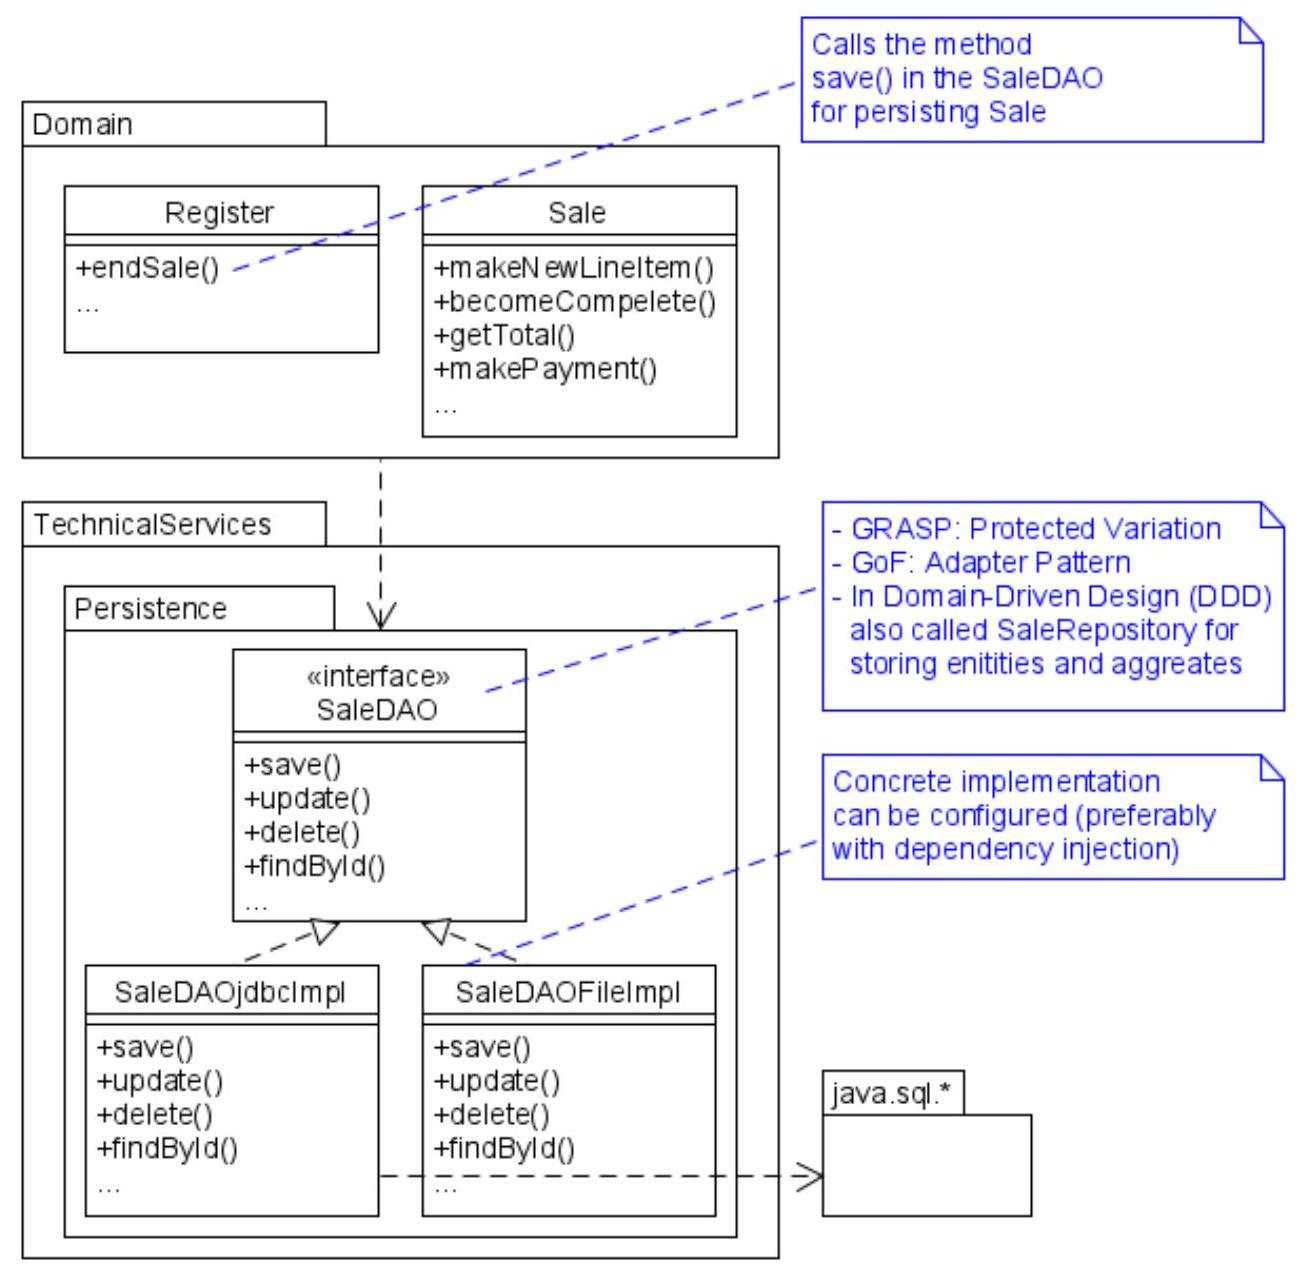
\includegraphics[width=\linewidth]{images/2025_01_02_5ba1dc702e9f94ba8e06g-14}
\end{itemize}

\section*{Verwendung eines O/R-Mappers (JPA mit Hibernate/Eclipselink o.a. Framework)}
\begin{itemize}
  \item Viel weniger Aufwand bzw. Code und standardisierte Schnittstelle
  \item Trennung von Fachlichkeit und Technik (Domänenklasse hat hohe Kohäsion)
  \item Gute Testbarkeit und Mocking der Persistenz
  \item DAO ist auch beim Einsatz von JPA empfehlenswert (Trennung von Fachlichkeit und Technik) - JPA könnte aber auch ohne DAO verwendet werden\\
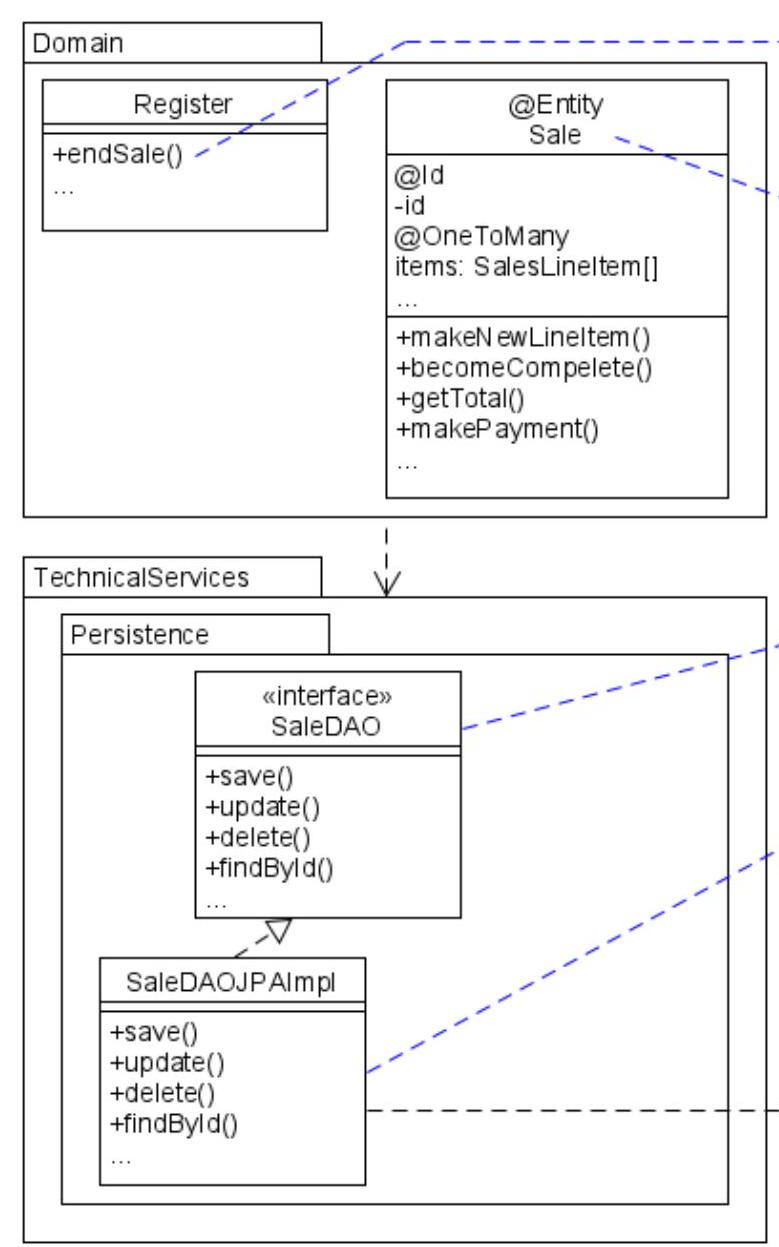
\includegraphics[width=\linewidth]{images/2025_01_02_5ba1dc702e9f94ba8e06g-15(1)}
\end{itemize}

Calls the method save() in the SaleDAO for persisting Sale

\begin{verbatim}
Same design pattems apply as for
\end{verbatim}

the option with handcrafted DAOs.

For implementing the DAO\\
the Java Persistence API the Java Persistence API (JPA) and a service provider (e.g. Hibernate) provide an orR mapping and the basic by using the annotations and a configuration file (persistence xml)For queries a Java Persistence Query Language (JPQL) is available.\\
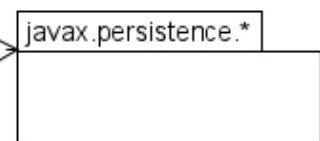
\includegraphics[width=\linewidth]{images/2025_01_02_5ba1dc702e9f94ba8e06g-15}

\begin{enumerate}
  \item Einführung in Persistenz
  \item Design-Optionen für Persistenz
  \item Persistenz mit JDBC
  \item O/R-Mapper mit DAO
  \item O/R-Mapper mit JPA
  \item Wrap-up und Ausblick
\end{enumerate}

\section*{Was genau ist JDBC?}
\begin{itemize}
  \item JDBC = Java Data Base Connectivity
  \item Standardisierte Schnittstelle, um auf relationale Datenbanken mit Hilfe von SQL zuzugreifen
  \item Cross-Plattform und DB-independent
  \item JDBC-API ist Teil der Java-Plattfrom seit JDK1.1 (1997)
  \item Die aktuelle Version ist 4.2\\
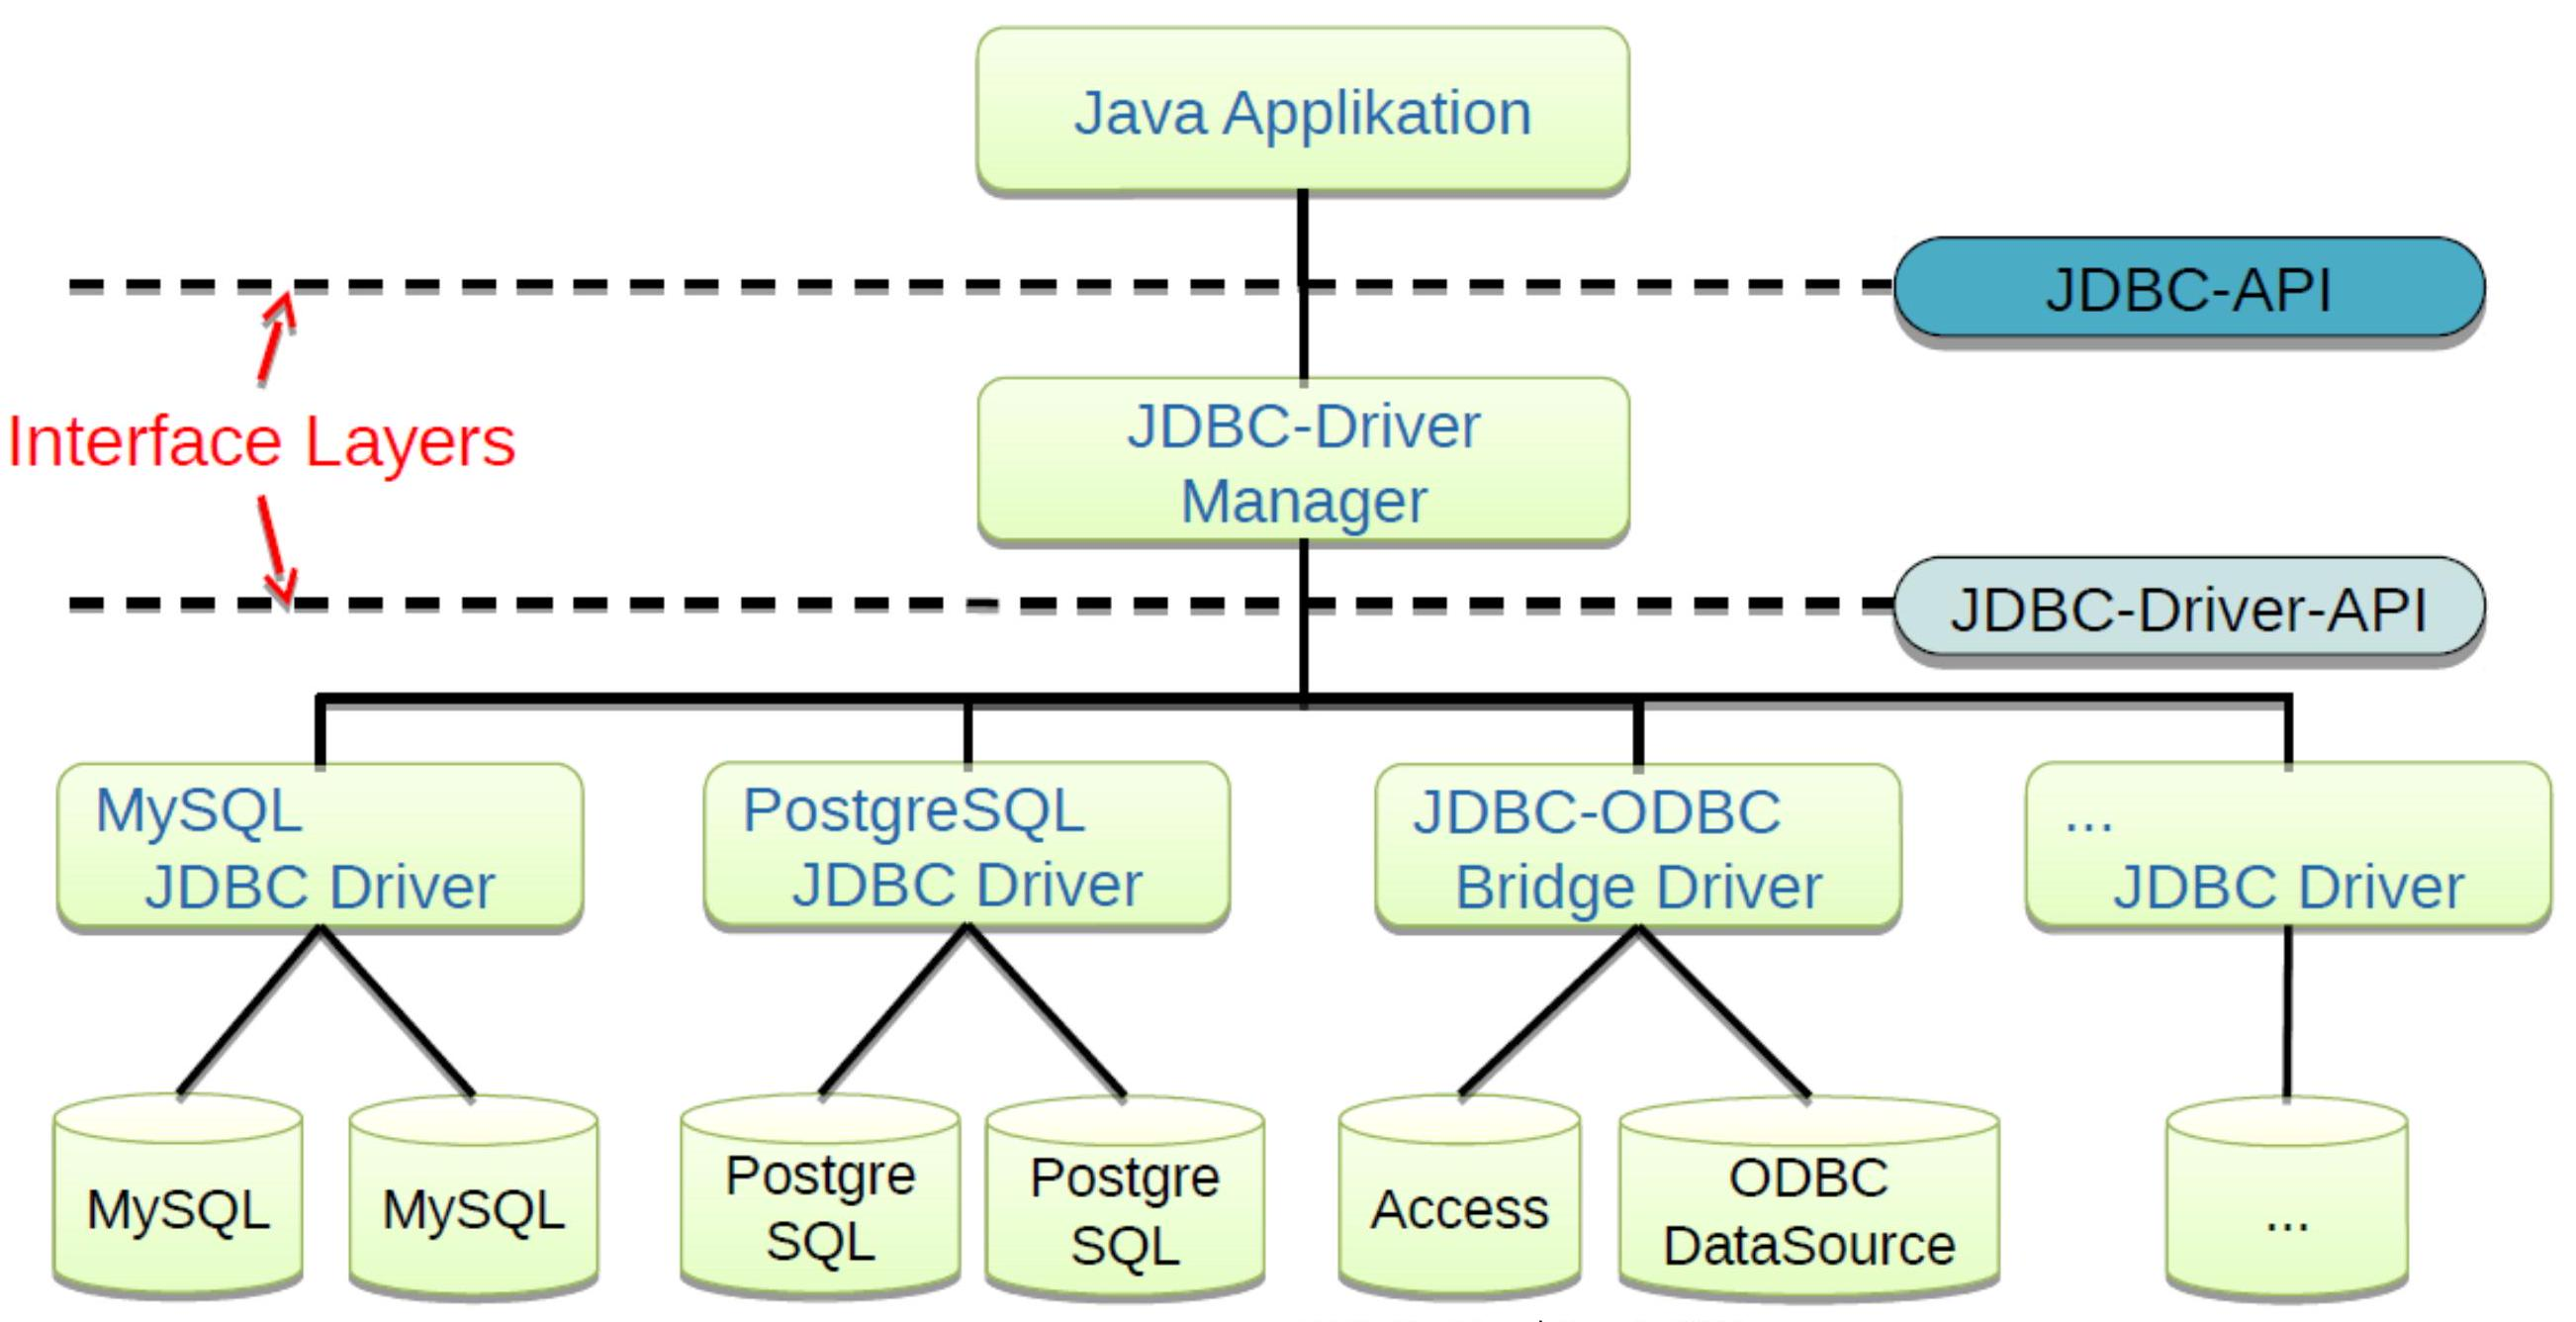
\includegraphics[width=\linewidth]{images/2025_01_02_5ba1dc702e9f94ba8e06g-18}
\end{itemize}

\section*{JDBC-API: Interfaces and Classes}
\begin{center}
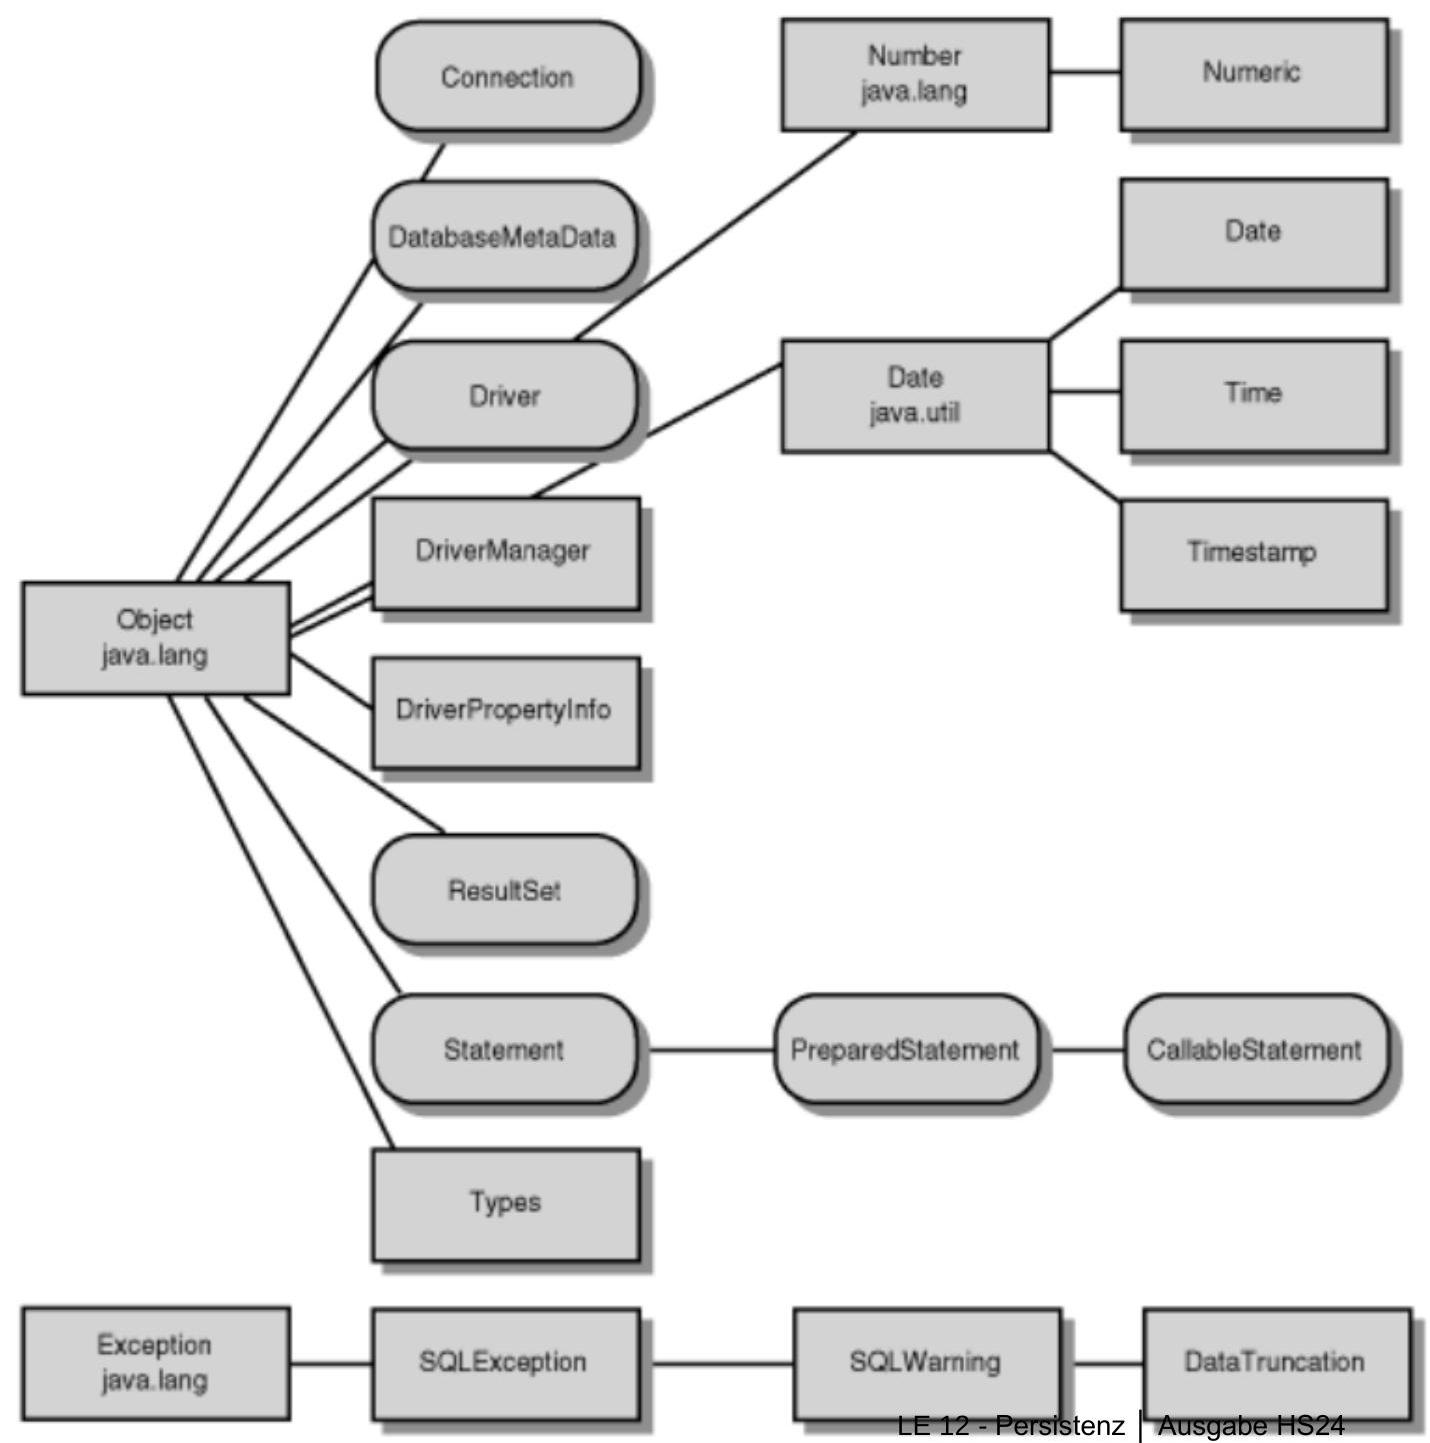
\includegraphics[width=\linewidth]{images/2025_01_02_5ba1dc702e9f94ba8e06g-19}
\end{center}

\section*{Anwendung von JDBC}
Basisanweisungen:

\begin{enumerate}
  \item Install and load JDBC driver
  \item Connect to SQL database
  \item Execute SQL statements
  \item Process query results
  \item Commit or Rollback DB updates
  \item Close Connection to database
\end{enumerate}

\begin{verbatim}
import java.sql.*;
public class DbTest {
    public static void main(String[] args)
        throws ClassNotFoundException, SQLException {
        Connection con = DriverManager.getConnection(
            "jdbc:postgresql://test.zhaw.ch/testdb",
            "user", "password");
        Statement st = con.createStatement();
        ResultSet rs = st.executeQuery(
            "SELECT * FROM test ORDER BY name");
        while (rs.next()) {
            System.out.println(
                "Column 1 contains '" +
                rs.getString(2) +"'");
        }
        con.close();
    }

  \end{verbatim}

1. Einführung in Persistenz
2. Design-Optionen für Persistenz
3. Persistenz mit JDBC
4. O/R-Mapping mit DAO
5. O/R-Mapping mit JPA
6. Wrap-up und Ausblick

\section*{O/R-Mapping Pattern}

Es sollen beide Varianten des O/R-Mapper Patterns anhand eines praktischen Beispiels betrachtet werden:
- DAO (Data Acess Object) ohne ein ORM (Object Relational Mapper)
- Umsetzung von DAO mit Hilfe von JPA (Java Persistence API)

\section*{DAO - Data Access Object Pattern}
- Das Artikel-Objekt repräsentiert das Domain-Model-Objekt.
- Die Verbindung zur Datenbank wird durch das DAO sichergestellt.
- Enthält die üblichen CRUD-Methoden wie create, read, update und delete.
- Kann auch Methoden enthalten wie findAll, findByName, findByID um eine Kollektion von Daten aus der Datenbank abzufragen.

\section*{DAO - Data Access Object Pattern}

School of
![](https://cdn.mathpix.com/cropped/2025_01_02_5ba1dc702e9f94ba8e06g-24.jpg?height=889&width=1795&top_left_y=508&top_left_x=676)

Das TransferObject aka. DTO kann zusätzlich für den Transport der Daten in einem verteilten System verwendet werden.

\section*{Beispiel Article und ArticleDAO}

School of Engineering

\section*{Business Object}


public class Article \{\\
private long id;\\
private String name;\\
private float price;\\
public long getId()\{\\
return id;\\
\}\\
public void setId(long id)\{\\
this id = id\\
\};\\
...\\
\}

\begin{verbatim}

\section*{Data Access Object (DAO)}
\end{verbatim}

//Interface to be implemented by all ArticleDAOs\\
public interface ArticleDAO \{\\
public void insert(Article item);\\
public void update(Article item);\\
public void delete(Article item);\\
public Article findById(int id);\\
public Collection<Article> findAll();\\
public Collection<Article> findByName (String name);\\
public Collection<Article> findByPrice (float price);\\
\}

\begin{verbatim}
1. Einführung in Persistenz
2. Design-Optionen für Persistenz
3. Persistenz mit JDBC
4. O/R-Mapping mit DAO
5. O/R-Mapping mit JPA
6. Wrap-up und Ausblick
\end{verbatim}

\section*{Versprechen von automatischem O/R-Mapping}
- Die Applikation wird von der DB entkoppelt
- Applikationsentwickler muss kein SQL beherrschen.
- Das relationale Modell der Datenbank hat keinen Einfluss auf das OO-Design.
- Automatische Persistenz
- Automatisierte Abbildung der Objekte in die relationalen Strukturen.
- Die Applikationsentwickler muss sich nicht um die «low-level»-Details kümmern.
- Transparente Persistenz / Persistence Ignorance
- Die Klassen des Domain-Models wissen nicht, dass sie persistiert und geladen werden können und haben keine Abhängigkeit zur Persistenz-Infrastruktur.
- JPA ist ein Java Standard für O/R-Mapping
- Verschiedene Implementationen, Hibernate vermutlich die bekannteste

\section*{JPA (Java Persistence API) Überblick}
- Es folgt eine kurze, unvollständige Auflistung der wichtigsten Konzepte von JPA.
- Starke Entkopplung der Anwendungslogik von der (relationalen) Datenbank.
- Die Domänenklassen sind ganz normale Java Klassen (POJO)
- Ausser Annotationen enthalten Sie keinen JPA spezifischen Code.
- Referenzen
- Werden entweder mit der referenzierenden Klasse (eager loading) oder erst, wenn die Referenz gebraucht wird (lazy loading), geladen.
- Referenzen können direkt traversiert werden, JPA erledigt das Laden des referenzierten Objekts im Hintergrund.
- Transaktionshandling und das Absetzen von Queries müssen über JPA spezifische Klassen abgewickelt werden.
- EntityManagerFactory, EntityManager, EntityTransaction

\section*{Technologie-Stack}
![](https://cdn.mathpix.com/cropped/2025_01_02_5ba1dc702e9f94ba8e06g-29.jpg?height=1166&width=745&top_left_y=476&top_left_x=146)

Java 5+

JPA Spezifikation
EclipseLink (TopLink), Hibernate, OpenJPA etc.
JDBC 4.0
Herstellerspezifisch
SQL (und Dialekte)

\section*{Entity Metadata}
- Kennzeichnung mit Annotation @Entity oder Mapping mit XML
- Klasse kann Basisklasse oder abgeleitet sein
- Klasse kann abstrakt oder konkret sein
- Serialisierbarkeit ist bezüglich Persistenz nicht erforderlich

\section*{Beispiel Entity}

School of
- Minimale Anforderung an eine Entity


@Entity\\
public class Employee \{\\
@Id\\
@GeneratedValue(strategy = GenerationType.IDENTITY)\\
private long id;\\
private String name;\\
private String lastName;

\begin{verbatim}
- Primärschlüssel können in Zusammenarbeit mit der Datenbank generiert werden. Strategien sind Identity, Table, Sequence und Auto
\end{verbatim}

@Entity public class Employee \{\\
@Id\\
@GeneratedValue(strategy = GenerationType.IDENTITY)\\
public Integer id;\\
\}\\
public class Employee \{\\
@TableGenerator(name = "Emp\_Gen", table = "ID\_GEN", pkColumnName = "GEN\_NAME",\\
valueColumnName = "GEN\_VAL")\\
@Id\\
@GeneratedValue(strategy = GenerationType.TABLE, generator = "Emp\_Gen")\\
private int id;



\section*{Parent-Child Beziehung}
![](https://cdn.mathpix.com/cropped/2025_01_02_5ba1dc702e9f94ba8e06g-33.jpg?height=367&width=1456&top_left_y=433&top_left_x=267)
- Mapping des Klassenmodells auf das DB-Schema mittels JPA: Metadata ist erforderlich.
- Je nach Klassenmodell wird entweder eine many-to-one Beziehung oder eine one-to-many Beziehung gemappt.
- Falls beide Richtungen gemappt werden sollen, so muss definiert werden, dass für beide derselbe Foreign-Key zugrunde liegt.
\begin{tabular}{|l|l|}
\hline \multicolumn{1}{|c|}{ Employee } \\
\hline id \\
\hline name \\
\hline salary \\
\hline department id \\
\hline
\end{tabular}

\section*{Ausblick Design Pattern Repository}
- Ein System mit einem komplexen Domänen-Model profitiert wie vorher beschrieben von einer Data-Mapper-Schicht (mit JPA und DAOs), um die Details des Datenbankzugriffcodes zu isolieren.
- Eine zusätzliche Abstraktionsschicht oberhalb des Data-Mappers kann helfen um die Konstruktion von Datenbank-Abfragen (Queries) an einem Ort zu konzentrieren.
- Diese zusätzliche Schicht wird um so wichtiger je mehr Domänen-Klassen vorhanden sind, die viele Zugriffe auf die Datenbank vornehmen.
- Die zusätzliche Schicht wird als Repository bezeichnet
- Das Konzept stammt aus Domain Driven Design, DDD (Eric Evans).
- Wird in den Wahlpflichtmodulen ASE1/2 anhand von Spring Data behandelt.

\section*{Design Pattern Repository: Schichtenmodell}
- 3-Tier Architecture
- Persistenz kann mittels Repositories umgesetzt werden
![](https://cdn.mathpix.com/cropped/2025_01_02_5ba1dc702e9f94ba8e06g-35.jpg?height=1179&width=1634&top_left_y=525&top_left_x=1581)

\section*{Idee und Beispiel Repository Pattern}

School of Engineering
InIT Institut für angewandte Informationstechnologie
- Eine Repository vermittelt zwischen Domänen- und Data-Mapping Schicht


9 [0/** * The GRASP controller for the use case process sale.\\
11 [*/\\
\textbackslash emptysetpublic class ProcessSaleHandler \{\\
private ProductDescriptionRepository catalog;\\
private SaleRepository saleRepository;\\
private Sale currentSale;\\
public ProcessSaleHandler(ProductDescriptionRepository catalog, SaleRepository saleRepository) \{\\
public void makeNewSale() \{\\
public void enterItem(String id, int quantity) \{\\
public Money getTotalOfSale() \{\\
@Transactional\\
public void endSale() \{\\
assert(currentSale != null \&\& !currentSale.isComplete());\\
this.currentSale.becomeComplete()\\
this.saleRepository.save(currentSale);\\
\}\\
public Money getTotalWithTaxesOfSale() \{\\
public void makePayment() \{

\begin{verbatim}
![](https://cdn.mathpix.com/cropped/2025_01_02_5ba1dc702e9f94ba8e06g-36.jpg?height=690&width=941&top_left_y=633&top_left_x=2285)
\end{verbatim}

曰/**\\
* Repository for Sale\\
* An implementation of CRUD and common search methods\\
* is automatically generated by Spring Data.\\
*/\\
6 @Repository\\
\textbackslash emptysetpublic interface SaleRepository extends CrudRepository<Sale, String>\\
public List<Sale> findOrderByDateTime();\\
public List<Sale> findByDateTime(final LocalDateTime dateTime);\\
L\}

\begin{verbatim}
1. Einführung in Persistenz
2. Design-Optionen für Persistenz
3. Persistenz mit JDBC
4. O/R-Mapping mit DAO
5. O/R-Mapping mit JPA
6. Wrap-up und Ausblick
- Viele Applikationen verlangen, dass Daten dauerhaft gesichert werden müssen nach dem Programmende.
- Bei kleineren Applikationen kann diese Persistenz auch selber ausprogrammiert werden.
- Dabei sollte aber das Design Pattern Data Access Object (DAO) oder Repository angewendet werden.
- Für grössere Applikationen werden heute sogenannte O/R-Mapper eingesetzt.
- Java bietet mit dem Java Persistence API (JPA) eine standardisierte Schnittstelle für das $O / R-M a p p i n g, ~ f u ̈ r ~ d i e ~ e s ~ v i e l e ~ P r o v i d e r ~ g i b t ~(z . B . ~ H i b e r n a t e) . ~$.

\section*{Ausblick}
- In der nächsten Lerneinheit werden wir:
- das Thema Design von Frameworks vertiefen.

\section*{Quellenverzeichnis}
[1] Oracle: Core J2EE Patterns - Data Access Object, https://www.oracle.com/java/technologies/dataaccessobject.html
[2] Oracle: Core J2EE Patterns - JPA,
https://www.oracle.com/java/technologies/persistence-jsp.html
[3] Hibernet: Documentation, https://hibernate.org/orm/documentation/5.4/
[4] Ranking Database: https://db-engines.com/en/ranking
\end{verbatim}


\end{document}